\documentclass[11pt,svgnames]{beamer}
\usepackage[english]{babel}
\usepackage[utf8]{inputenc}
\usepackage{amsmath,amsthm,amsfonts}
\usepackage{xcolor}
\usepackage{enumerate}
\usepackage{graphicx}
\usepackage{float}
\usepackage{epstopdf}
\usepackage{tcolorbox}
%##############################################################################################################################
\usetheme{Madrid}
\usecolortheme[named=black]{structure}
\usefonttheme{structurebold}
%##############################################################################################################################
\renewcommand{\comment}[1]{}
\renewcommand{\kappa}{\mathsf k}
\newcommand{\Esse}{\mathcal S}
\newcommand{\Elle}{\mathtt L}
\newcommand{\Ee}{\mathtt E}
\newcommand{\enne}{\mathfrak n}
\newcommand{\di}{\mathtt d}
\newcommand{\Enne}{\mathcal N}
\newcommand{\emme}{\mathfrak m}
\newcommand{\elle}{\mathnormal l}
%\setbeamertemplate{footline}[frame number]%##############################################################################################################################
\title[Models for inheritance in OO languages]{\huge Models for hierarchical \\ inheritance structures in \\ object-oriented programming \\ languages}
\author[Mariacristina Romano]{\vphantom{a} \\ \huge Mariacristina Romano \\ \vphantom{a} }
\institute[]{\small{\sc Università degli studi di Milano} \\
\tiny
{\sc Facoltà di Scienze e Tecnologie} \\
{\it Corso di laurea magistrale in Fisica}}
\date{15 aprile 2015}
%##############################################################################################################################
\begin{document}
 \beamertemplatenavigationsymbolsempty
%--------------------------------------------------------------
\begin{frame}[plain,noframenumbering]
\titlepage
\end{frame}

%--------------------------------------------------------------
\begin{frame}[t]{Introduction}
\begin{tcolorbox}[colframe=PowderBlue]
\center
Complex Systems and Computer science
\end{tcolorbox}
\end{frame}
%--------------------------------------------------------------
\begin{frame}[t,noframenumbering]{Introduction}
\begin{tcolorbox}[colframe=PowderBlue]
\center
Complex Systems and Computer science
\end{tcolorbox}
\vspace{0.3cm}
\begin{tcolorbox}[colframe=Aqua]
\center
Object-oriented paradigm
\end{tcolorbox}
\end{frame}
%--------------------------------------------------------------
\begin{frame}[t,noframenumbering]{Introduction}
\begin{tcolorbox}[colframe=PowderBlue]
\center
Complex Systems and Computer science
\end{tcolorbox}
\vspace{0.3cm}
\begin{tcolorbox}[colframe=Aqua]
\center
Object-oriented paradigm
\end{tcolorbox}
\vspace{0.3cm}
\begin{tcolorbox}[colframe=DeepSkyBlue]
\center
Inheritance
\end{tcolorbox}
\end{frame}
%--------------------------------------------------------------
\begin{frame}[t,noframenumbering]{Introduction}
\begin{tcolorbox}[colframe=PowderBlue]
\center
Complex Systems and Computer science
\end{tcolorbox}
\vspace{0.3cm}
\begin{tcolorbox}[colframe=Aqua]
\center
Object-oriented paradigm
\end{tcolorbox}
\vspace{0.3cm}
\begin{tcolorbox}[colframe=DeepSkyBlue]
\center
Inheritance
\end{tcolorbox}
\vspace{0.3cm}
\begin{tcolorbox}[colframe=DodgerBlue]
\center
Code reuse
\end{tcolorbox}
\end{frame}
%--------------------------------------------------------------
\begin{frame}[t,noframenumbering]{Introduction}
\begin{tcolorbox}[colframe=PowderBlue]
\center
Complex Systems and Computer science
\end{tcolorbox}
\vspace{0.3cm}
\begin{tcolorbox}[colframe=Aqua]
\center
Object-oriented paradigm
\end{tcolorbox}
\vspace{0.3cm}
\begin{tcolorbox}[colframe=DeepSkyBlue]
\center
Inheritance
\end{tcolorbox}
\vspace{0.3cm}
\begin{tcolorbox}[colframe=DodgerBlue]
\center
Code reuse
\end{tcolorbox}
\vspace{0.3cm}
\begin{tcolorbox}[colframe=RoyalBlue]
\center
Hierarchies
\end{tcolorbox}
\end{frame}
%--------------------------------------------------------------
\comment{
\begin{frame}{Object-oriented programming languages}{Introduction}
Object-oriented programming is a paradigm that allows an intelligent \textbf{\underline{code reuse}} through inheritance and polymorphism.

\vspace{0.3cm}
Through the concept of objects, we can consider each program as an ensemble of many small elements which interact and cooperate to achieve the same goal, that is the purpose for which each program has been made: a \textbf{\underline{complex system}}!

\vspace{0.3cm}
One of the most important relation that can links objects is the \textbf{\underline{inheritance}}: a rule introduced in object-oriented programming languages in order to facilitate and make automatic the reuse of code.

\vspace{0.3cm}
Inheritance allows the construction of \textbf{\underline{multilevel hierarchies}}, which can be modeled by directed acyclic graphs.
%
%\vspace{0.3cm}
%\begin{tcolorbox}[colframe=green]
%\center
%Which kind of graphs arise from hierarchical relations?
%\end{tcolorbox}
\end{frame}
} 
%--------------------------------------------------------------
\begin{frame}{Example of inheritance hierarchy}{Data Analysis - Project Soomla Cocos2dx}
\begin{figure}[H]%
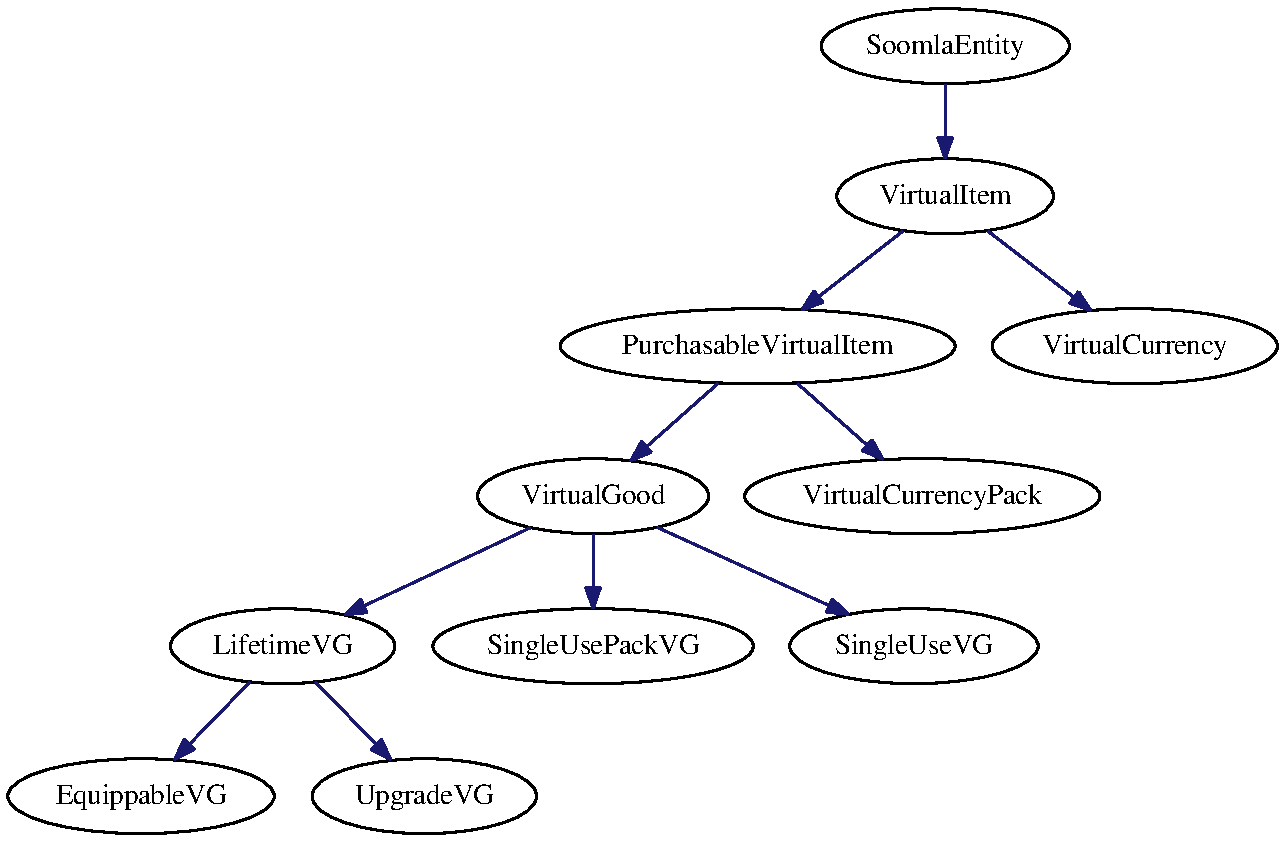
\includegraphics[width=11cm,draft=false]{immagini/soomla1.pdf}
\end{figure}
\end{frame}

%--------------------------------------------------------------
\begin{frame}{Noisy complex system dataset}{Data Analysis - dataset}
Packages have been downloaded from \textbf{\underline{GitHub}}, the actual largest code host on the web.

\vspace{0.5cm}
To give a \textbf{\underline{complete overview}} of inheritance hierarchies, three different programming languages have been analyzed.

\vspace{0.5cm}
The \textbf{\underline{dataset}} contains:
\begin{itemize}
\item 17333 C++ projects (3233447 hierarchies)
\item 25318 Java projects (3504681 hierarchies)
\item 20010 Python projects (2491603 hierarchies)
\end{itemize}
\vspace{0.2cm}
\begin{tcolorbox}[colframe=green]
\center
Almost 10 millions of inheritance hierarchies!
\end{tcolorbox}
\end{frame}

%--------------------------------------------------------------
\begin{frame}{Depth VS Size is logarithmic}{Data Analysis}
\begin{tcolorbox}[colframe=red]
\center
 C++
\end{tcolorbox}
\begin{figure}[p]%
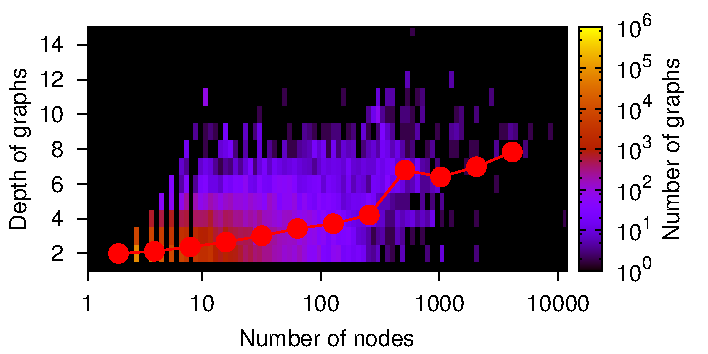
\includegraphics[width=12cm,draft=false]{immagini/mapcpp.pdf}
\end{figure}
\end{frame}

%--------------------------------------------------------------
\begin{frame}[noframenumbering]{Depth VS Size is logarithmic}{Data Analysis}
\begin{tcolorbox}[colframe=green]
\center
 Java
\end{tcolorbox}
\begin{figure}[p]%
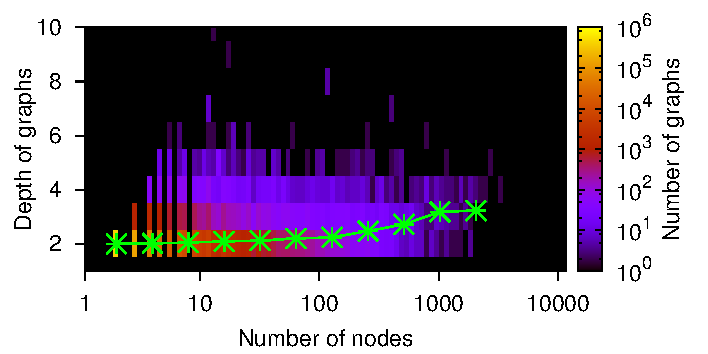
\includegraphics[width=12cm,draft=false]{immagini/mapjava.pdf}
\end{figure}

\end{frame}

%--------------------------------------------------------------
\begin{frame}[noframenumbering]{Depth VS Size is logarithmic}{Data Analysis}
\begin{tcolorbox}[colframe=blue]
\center
 Python
\end{tcolorbox}
\begin{figure}[p]%
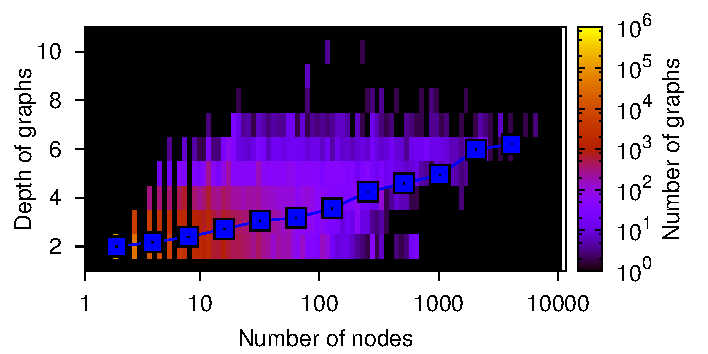
\includegraphics[width=12cm,draft=false]{immagini/mappy.pdf}
\end{figure}
\end{frame}

%--------------------------------------------------------------
\begin{frame}{Depth VS Size is logarithmic}{Data Analysis - Comparison among languages}
\begin{figure}[H]%
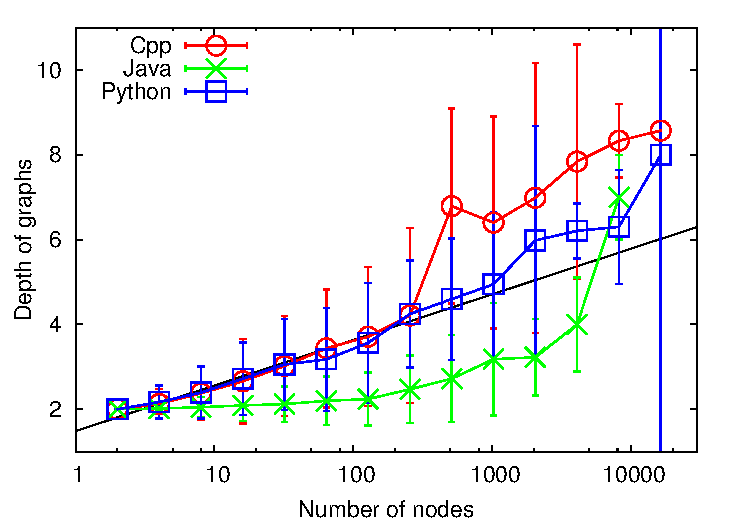
\includegraphics[width=10cm,draft=false]{immagini/depVSNnodes_err.pdf}
\end{figure}
\end{frame}

%--------------------------------------------------------------
\begingroup
\setbeamercolor{background canvas}{bg=black}
\begin{frame}[plain,noframenumbering]
\center
\textbf {\Huge {\color{white} {Sharing Tree model}}}

\vspace{0.5cm}
\textbf {\large {\color{white} {(A microscopic model)}}}
\end{frame}
\endgroup

%--------------------------------------------------------------
\begin{frame}{How to build the structure}{Sharing Tree model (microscopic model)}
\begin{figure}[p]%
\center
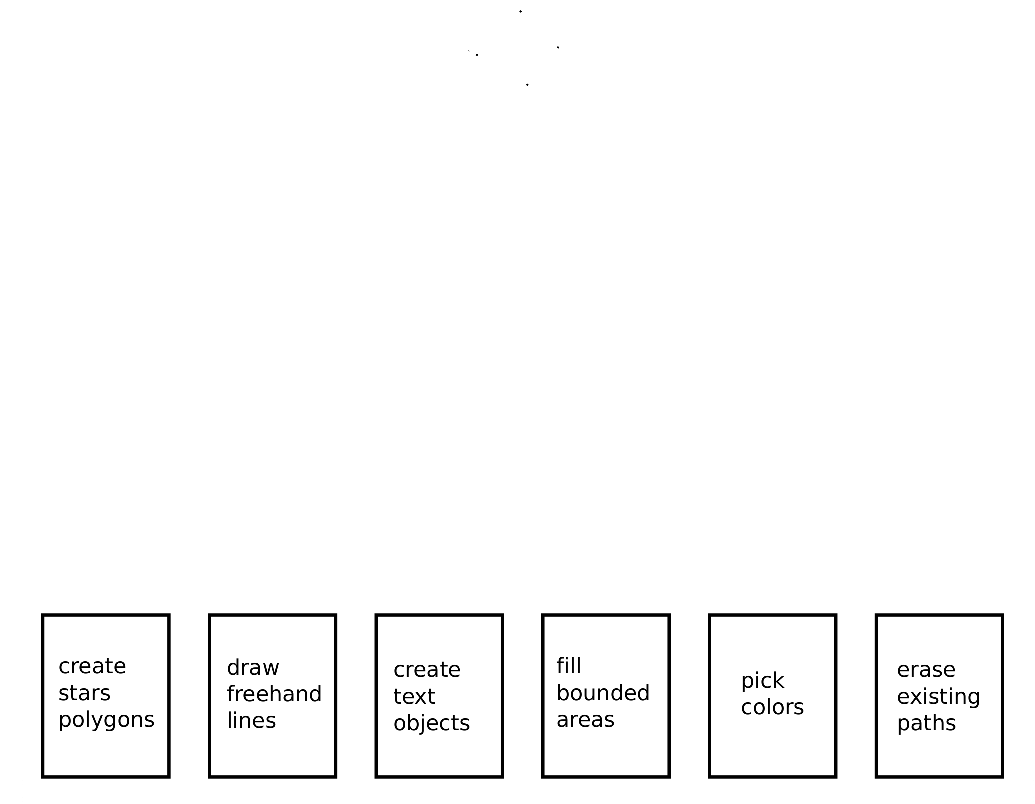
\includegraphics[width=8cm,draft=false]{immagini/a1.pdf}
\end{figure}
\end{frame}
\begin{frame}[noframenumbering]{How to build the structure}{Sharing Tree model (microscopic model)}
\begin{figure}[p]%
\center
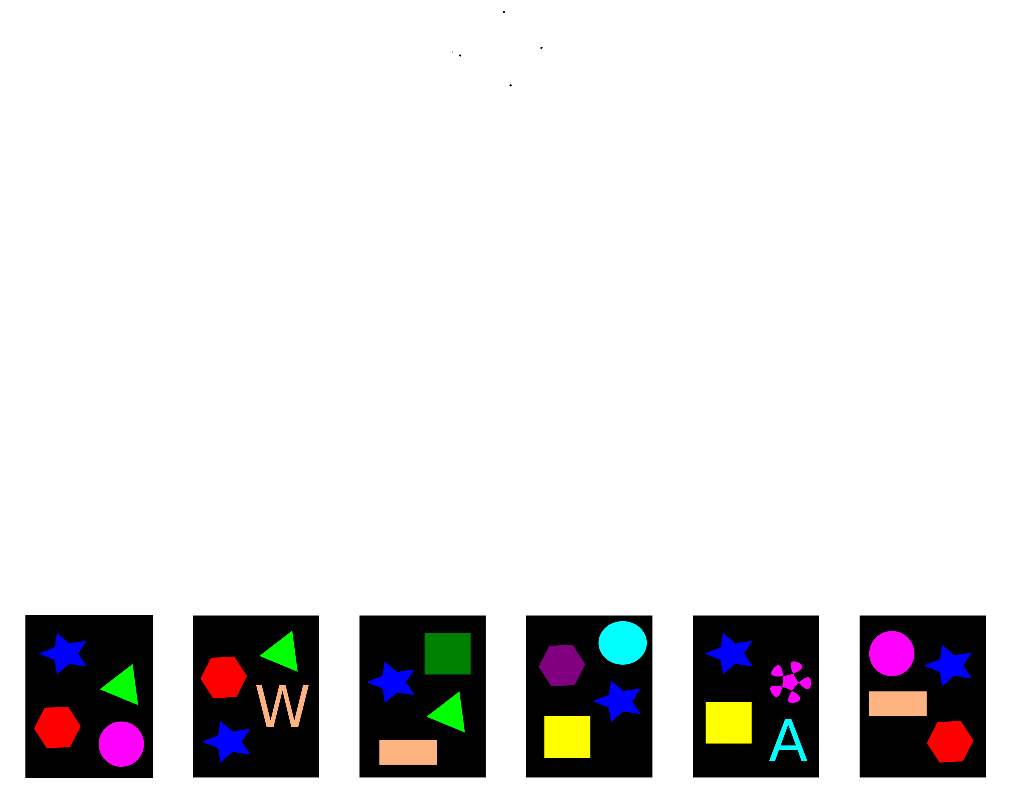
\includegraphics[width=8cm,draft=false]{immagini/a2.pdf}
\end{figure}
\end{frame}
\begin{frame}[noframenumbering]{How to build the structure}{Sharing Tree model (microscopic model)}
\begin{figure}[p]%
\center
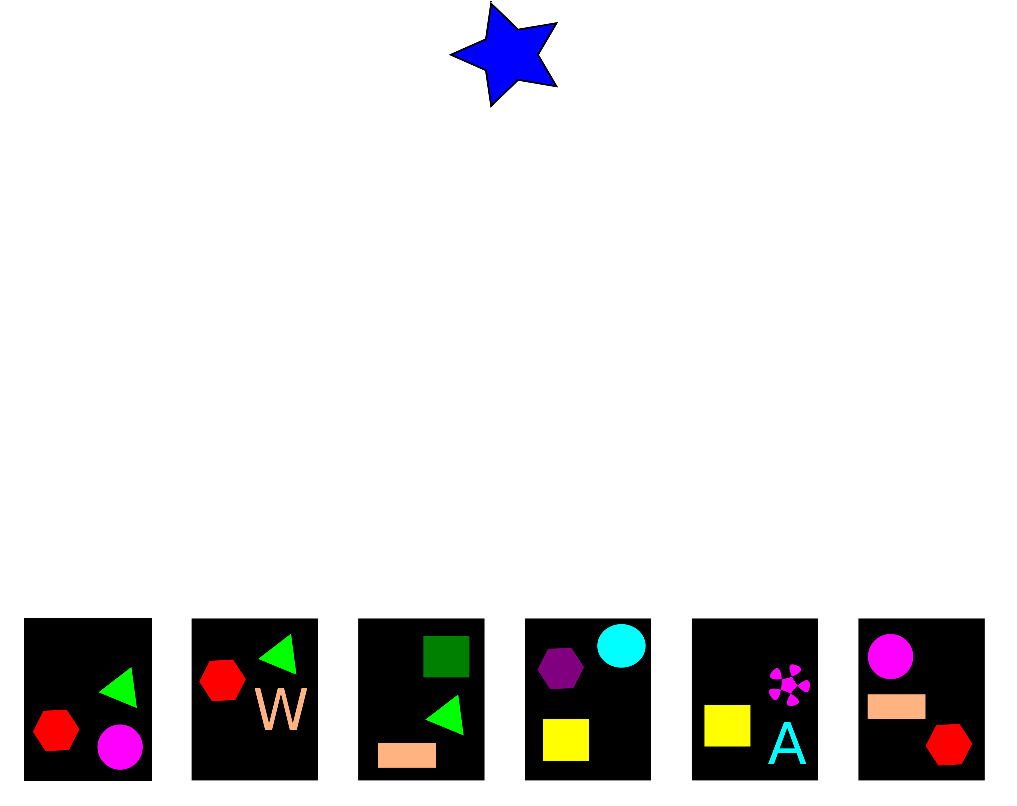
\includegraphics[width=8cm,draft=false]{immagini/aa3.pdf}
\end{figure}
\end{frame}
\begin{frame}[noframenumbering]{How to build the structure}{Sharing Tree model (microscopic model)}
\begin{figure}[p]%
\center
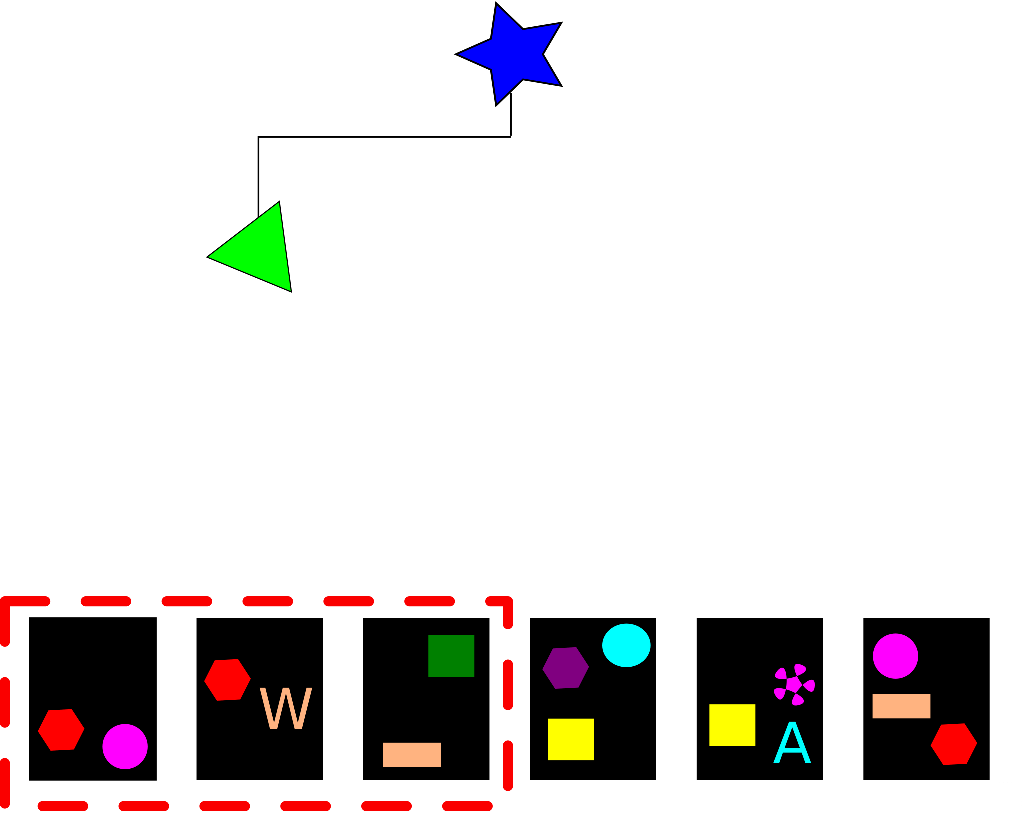
\includegraphics[width=8cm,draft=false]{immagini/aa4.pdf}
\end{figure}
\end{frame}
\begin{frame}[noframenumbering]{How to build the structure}{Sharing Tree model (microscopic model)}
\begin{figure}[p]%
\center
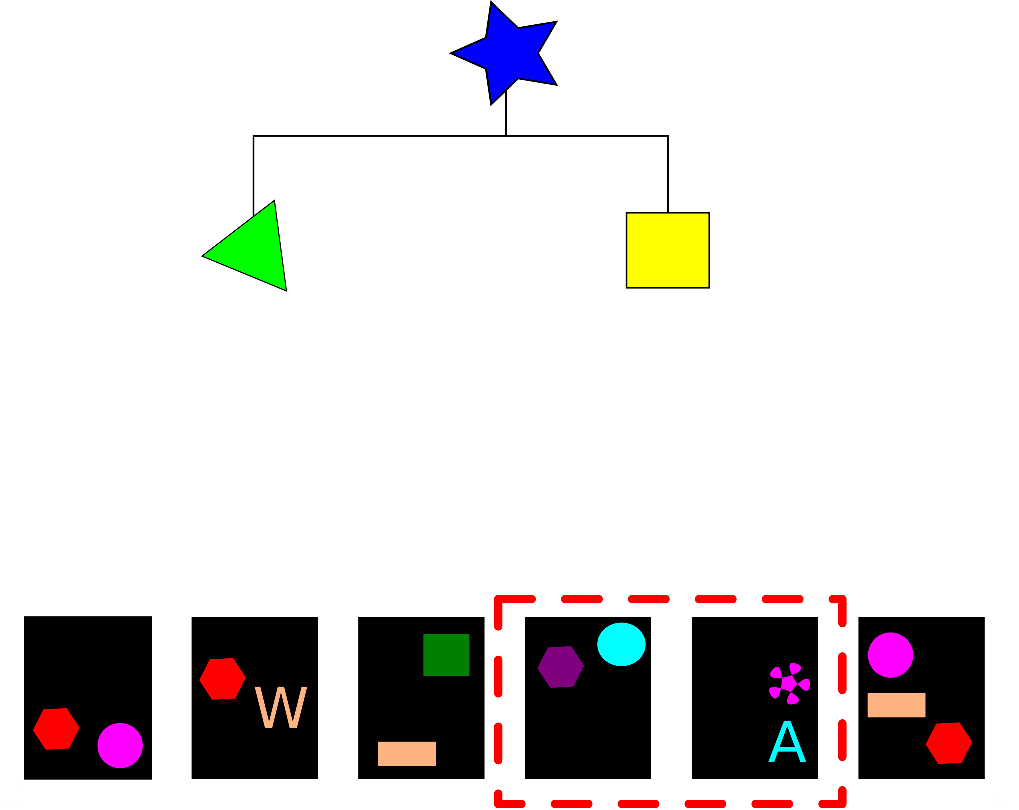
\includegraphics[width=8cm,draft=false]{immagini/aa5.pdf}
\end{figure}
\end{frame}
\begin{frame}[noframenumbering]{How to build the structure}{Sharing Tree model (microscopic model)}
\begin{figure}[p]%
\center
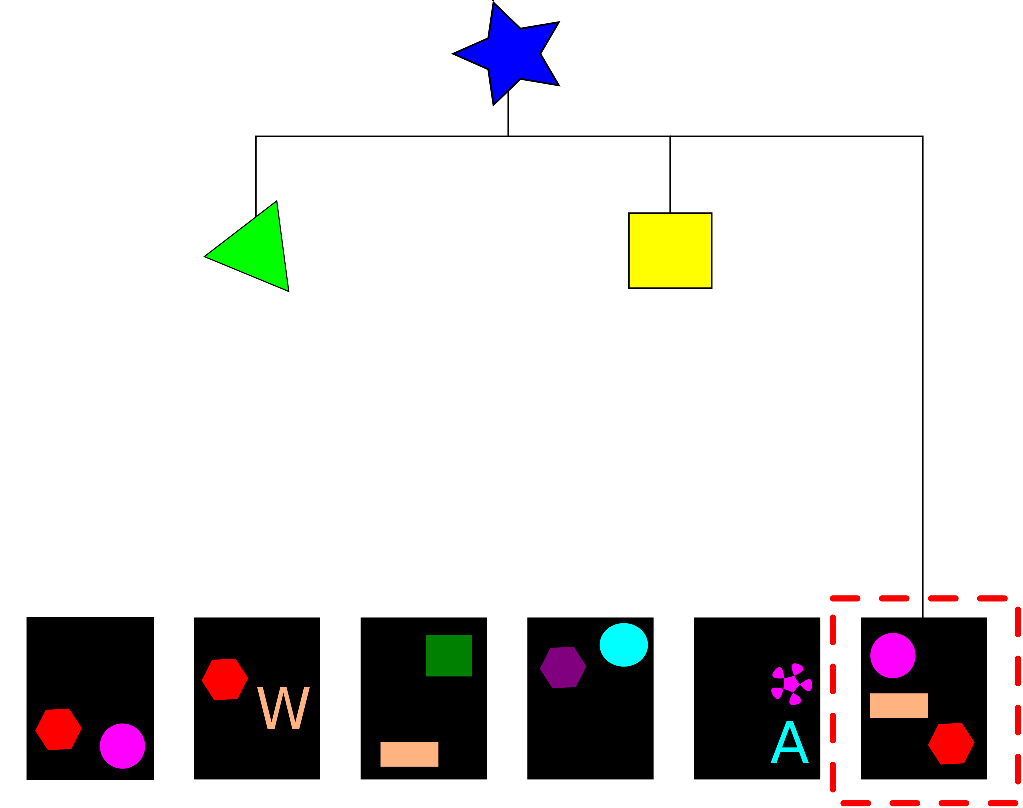
\includegraphics[width=8cm,draft=false]{immagini/aa6.pdf}
\end{figure}
\end{frame}
\begin{frame}[noframenumbering]{How to build the structure}{Sharing Tree model (microscopic model)}
\begin{figure}[p]%
\center
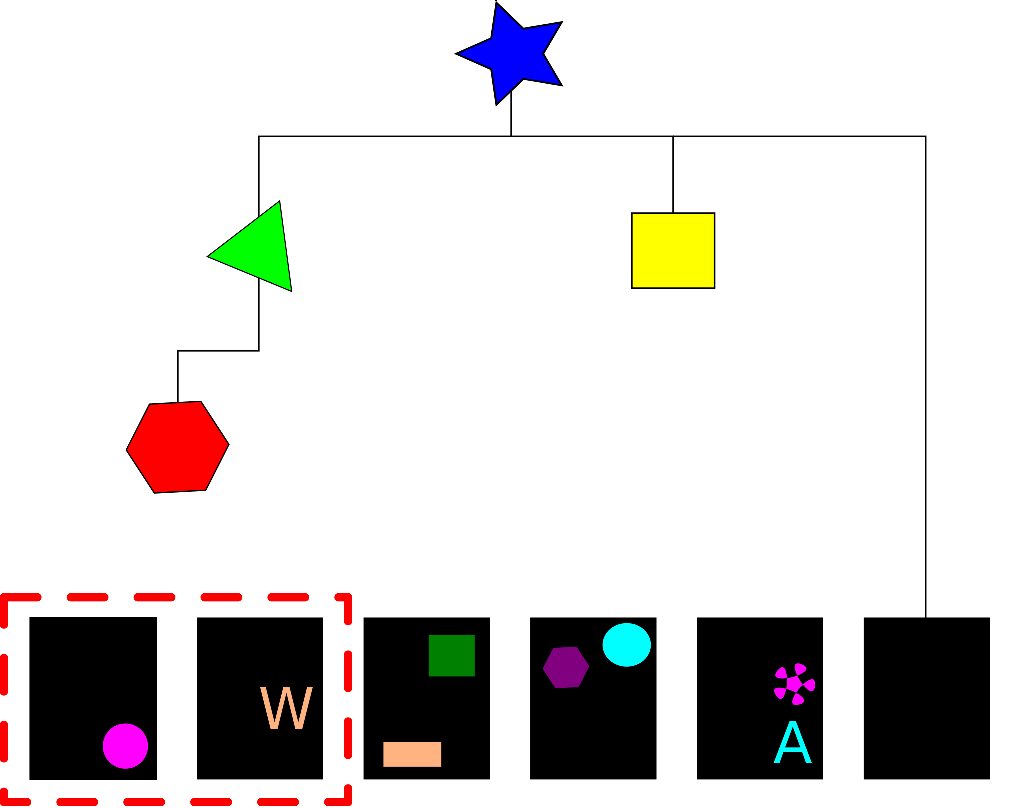
\includegraphics[width=8cm,draft=false]{immagini/aa7.pdf}
\end{figure}
\end{frame}

\begin{frame}[noframenumbering]{How to build the structure}{Sharing Tree model (microscopic model)}
\begin{figure}[p]%
\center
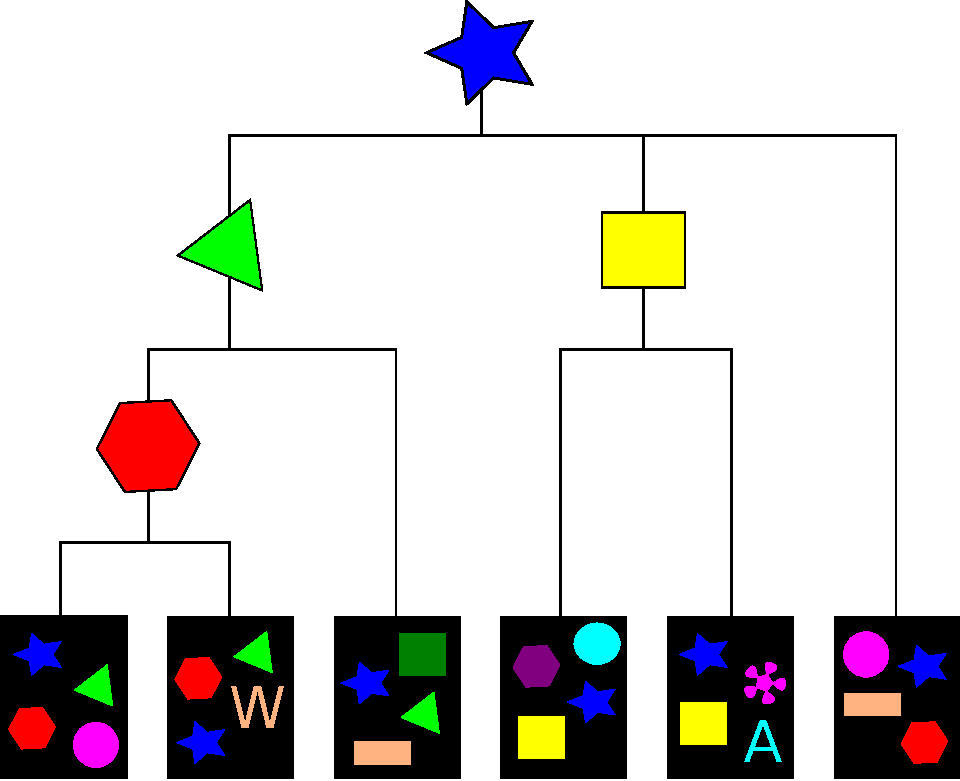
\includegraphics[width=8cm,draft=false]{immagini/sharingtree.pdf}
\end{figure}
\end{frame}

%--------------------------------------------------------------
\begin{frame}{Depth VS Size is logarithmic}{Sharing Tree model (microscopic model)}
\begin{figure}[p]%
\center
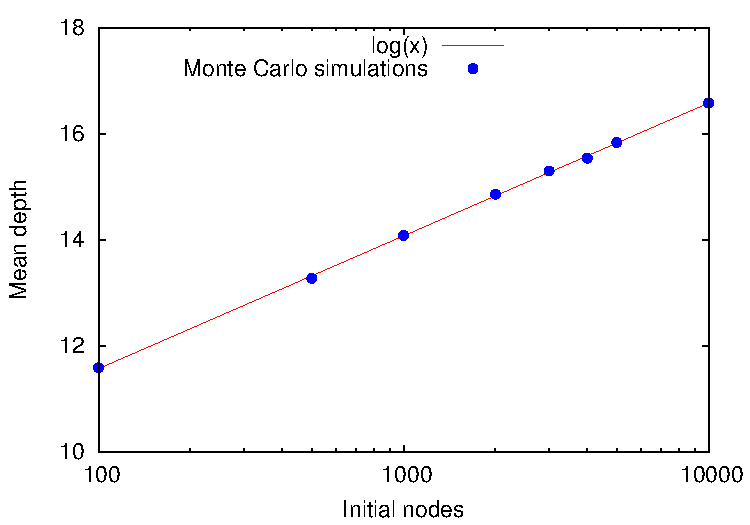
\includegraphics[width=10cm,draft=false]{immagini/depVSNnodes_tree.pdf}
\end{figure}
\end{frame}

%--------------------------------------------------------------
\begingroup
\setbeamercolor{background canvas}{bg=black}
\begin{frame}[plain,noframenumbering]
\center
\textbf {\Huge {\color{white} {Minimal Effort model}}}

\vspace{0.5cm}
\textbf {\large {\color{white} {(A mean field model)}}}
\end{frame}
\endgroup
%--------------------------------------------------------------
\begin{frame}[t]{The Effort to build a hierarchy}{Minimal Effort model (mean field model)}
\begin{tcolorbox}[colframe=green]
\[ \Ee = \sum_{\sigma}^{\Enne} \text{cost}(\sigma) \]
\end{tcolorbox}
\end{frame}

%--------------------------------------------------------------
\begin{frame}[noframenumbering]{You need $\boldsymbol{\enne}$ classes to perform a task}{Minimal Effort model (mean field model)}
\begin{figure}[H]%
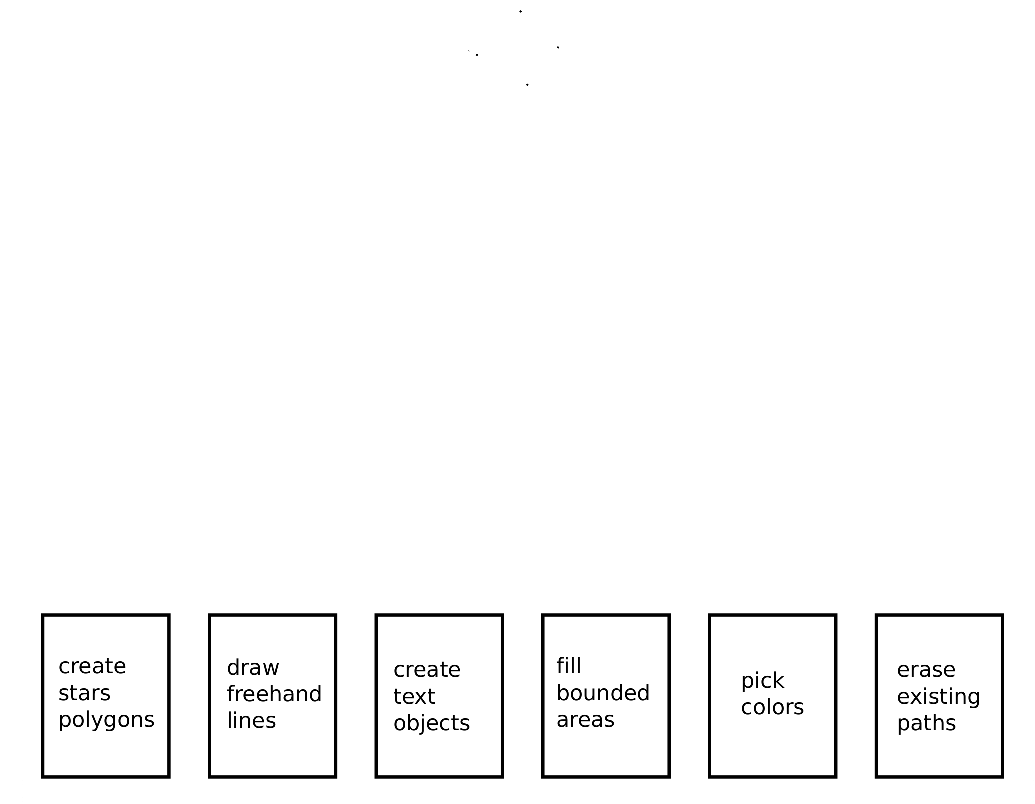
\includegraphics[width=9cm,draft=false]{immagini/a1.pdf}
\end{figure}
\end{frame}

%--------------------------------------------------------------
\begin{frame}[noframenumbering]{The cost of each class}{Minimal Effort model (mean field model)}
\begin{figure}[H]%
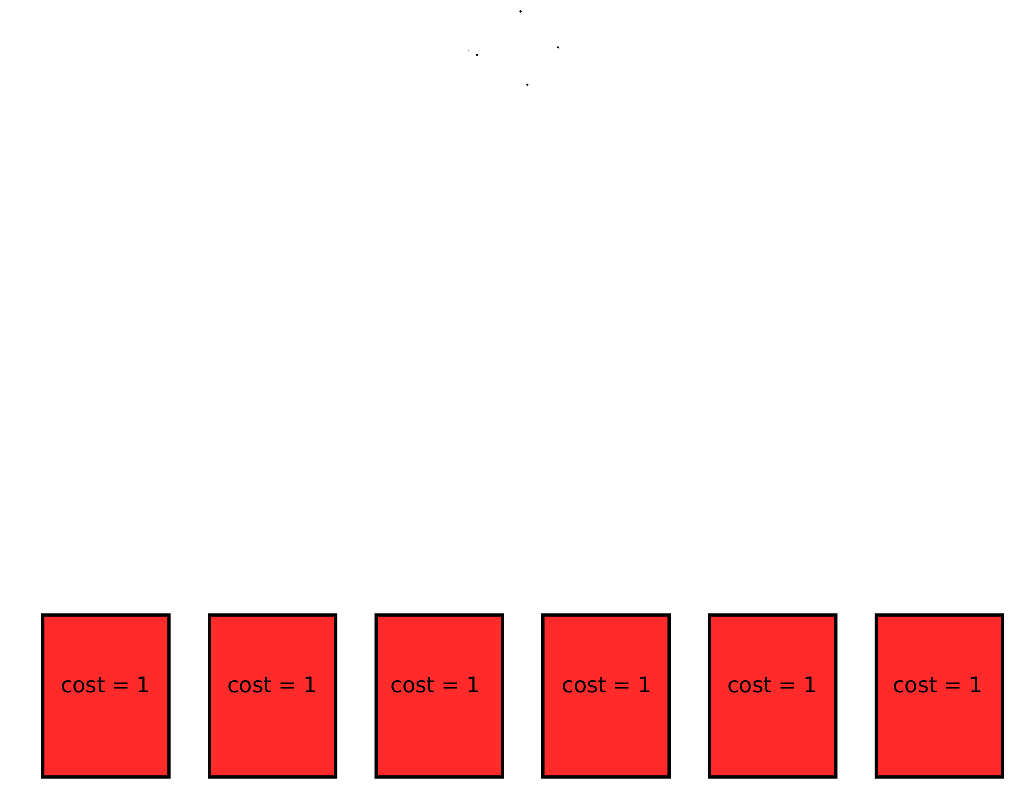
\includegraphics[width=9cm,draft=false]{immagini/aaa.pdf}
\end{figure}
\end{frame}

%--------------------------------------------------------------
\begin{frame}[noframenumbering]{Reuse}{Minimal Effort model (mean field model)}
\begin{figure}[H]%
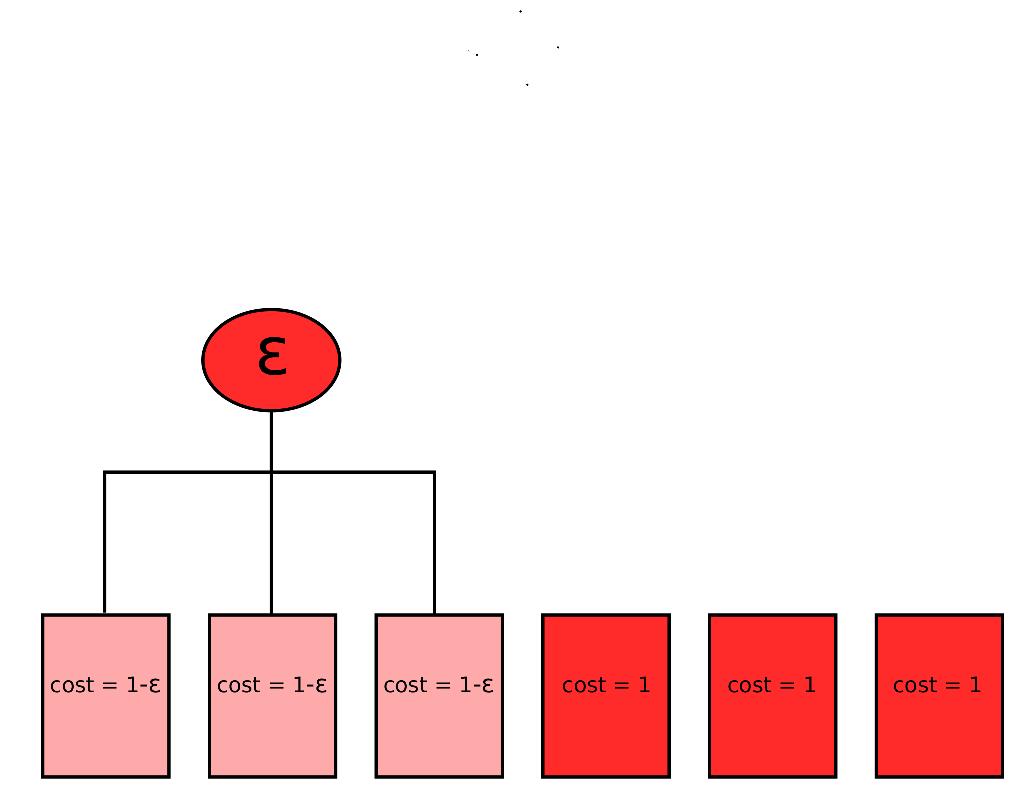
\includegraphics[width=9cm,draft=false]{immagini/bbb.pdf}
\end{figure}
\end{frame}

%--------------------------------------------------------------
\begin{frame}[noframenumbering]{Competition}{Minimal Effort model (mean field model)}
\begin{figure}[H]%
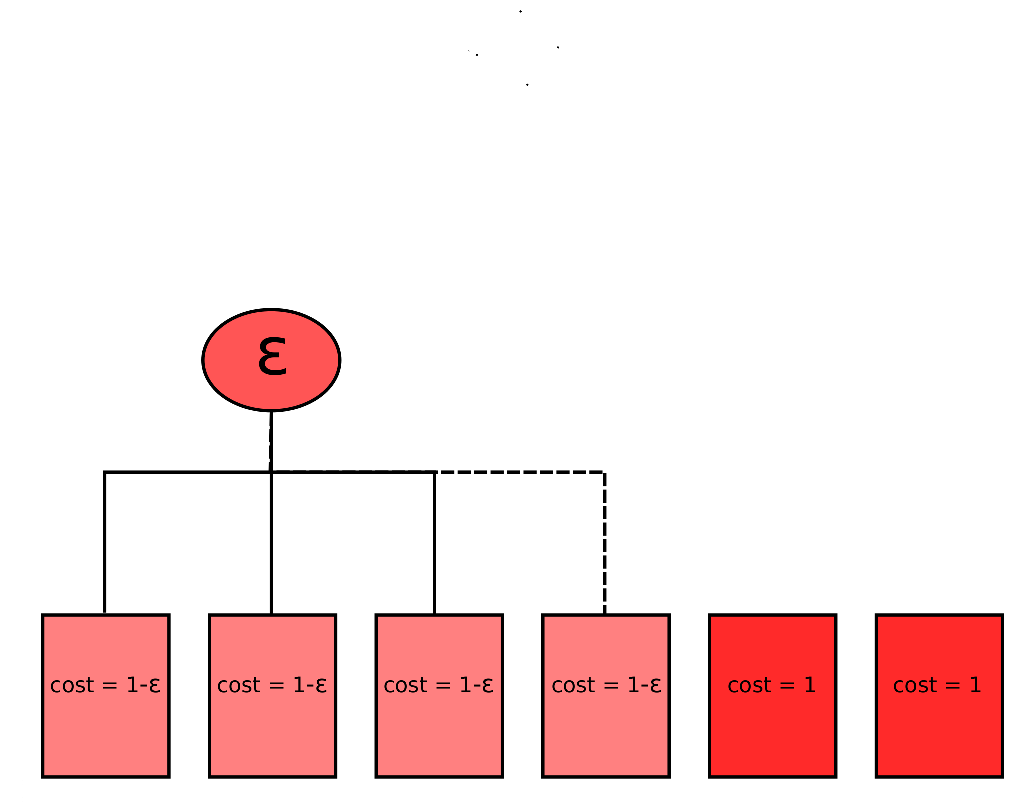
\includegraphics[width=9cm,draft=false]{immagini/ccc.pdf}
\end{figure}
\end{frame}

%--------------------------------------------------------------
\begin{frame}[t]{Competition}{Minimal Effort model (mean field model)}
\[ \Ee = \sum_{\sigma}^{\Enne} \text{cost}(\sigma) \]
\begin{tcolorbox}[colframe=green]
\[ \Ee = \sum_{\sigma}^{\Enne} \left[1 - \varepsilon(\emme) \right]\]
\end{tcolorbox}
\end{frame}

%--------------------------------------------------------------
\begin{frame}[noframenumbering]{The effort of ``writing'' a tree}{Minimal Effort model (mean field model)}
\begin{figure}[H]%
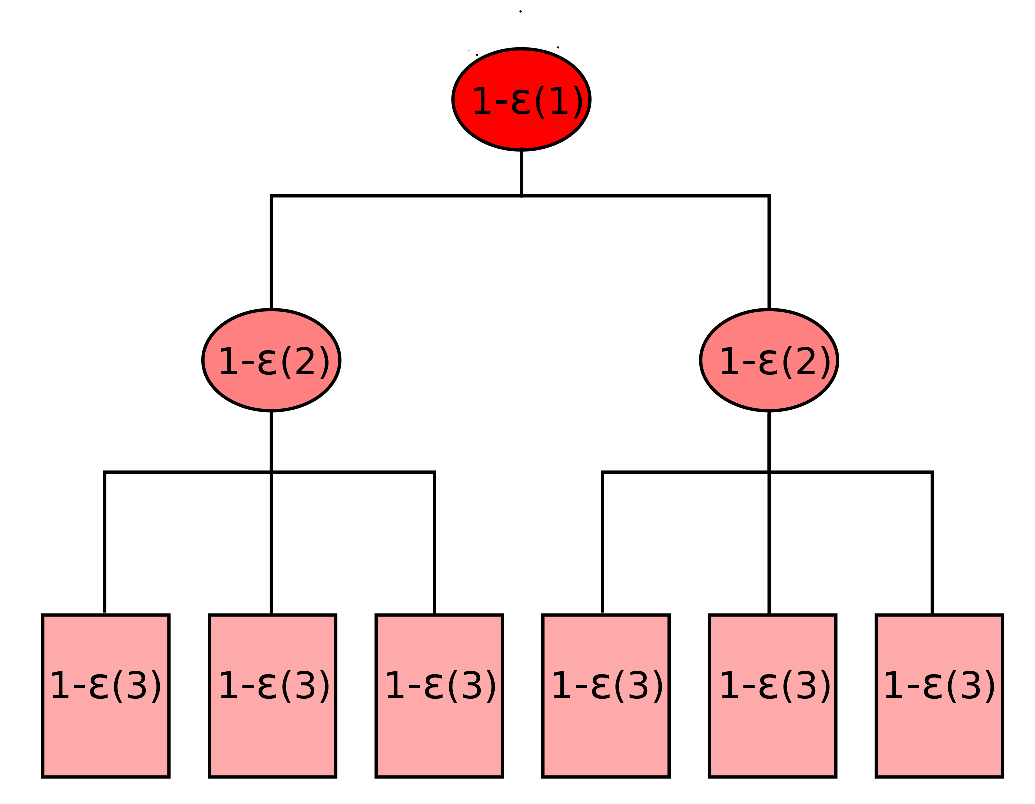
\includegraphics[width=9cm,draft=false]{immagini/ddd.pdf}
\end{figure}
\end{frame}


%#######################################################################################################
\begin{frame}[t,noframenumbering]{How much of the code is shareable?}{Minimal Effort model (mean field model)}
The probability to find a selected symbol in a sequence of $\kappa$ extractions is
\[ p = 1 - \left ( 1 -\frac{1}{\Esse} \right )^\kappa \]
\end{frame}
%--------------------------------------------------------------
\begin{frame}[t,noframenumbering]{How much of the code is shareable?}{Minimal Effort model (mean field model)}
The probability to find a selected symbol in a sequence of $\kappa$ extractions is
\[ p = 1 - \left ( 1 -\frac{1}{\Esse} \right )^\kappa \]
\vspace{1.5cm}
\small
\[\Esse \to \infty \qquad \kappa \to \infty \qquad \beta \equiv \frac{\kappa}{\Esse} \qquad e^{-\beta}= \lim_{\Esse \to +\infty} \left( 1 - \frac{1}{\Esse} \right)^{\beta \Esse}\]
\normalsize
\end{frame}
%--------------------------------------------------------------
\begin{frame}[t,noframenumbering]{How much of the code is shareable?}{Minimal Effort model (mean field model)}
The probability to find a selected symbol in a sequence of $\kappa$ extractions is
\[ p = 1 - \left ( 1 -\frac{1}{\Esse} \right )^\kappa \]

The probability to find the symbol in $\emme$ independent sets
\[ p = 1 - e^{-\beta} \qquad \to \qquad \rho = \left(1 - e^{-\beta}\right)^{\emme}\]
\end{frame}
%--------------------------------------------------------------
\begin{frame}[t,noframenumbering]{How much of the code is shareable?}{Minimal Effort model (mean field model)}
The probability to find a selected symbol in a sequence of $\kappa$ extractions is
\[ p = 1 - \left ( 1 -\frac{1}{\Esse} \right )^\kappa \]

The probability to find the symbol in $\emme$ independent sets
\[ p = 1 - e^{-\beta} \qquad \to \qquad \rho = \left(1 - e^{-\beta}\right)^{\emme}\]

\vspace{0.5cm}
\Large The \underline{\textbf{shareable code}} is \normalsize
\[ \varepsilon (\emme) = \frac{\Esse}{\kappa} \left(1 - e^{-\beta}\right)^{\emme} = \frac{1}{\beta} \left(1 - e^{-\beta}\right)^{\emme} \equiv e^{-\alpha \emme}\]

\end{frame}

%--------------------------------------------------------------
\begin{frame}[t]{The shared code}{Minimal Effort model (mean field model)}
\[ \Ee = \sum_{\sigma}^{\Enne} \text{cost}(\sigma) \]
\[ \Ee = \sum_{\sigma}^{\Enne} \left[ 1 - \varepsilon(\emme) \right] \]
\begin{tcolorbox}[colframe=green]
\[ \Ee = \sum_{\sigma}^{\Enne} \left[1 - e^{-\alpha \emme} \right] \]
\end{tcolorbox}
\end{frame}

%--------------------------------------------------------------
\begin{frame}[noframenumbering]{Mean field approach}{Minimal Effort model (mean field model)}
The \underline{\textbf{number of nodes}} at each level
\[ \{ \enne(\elle) \}_{\elle=1}^{\Elle} = \{ \enne(1), \enne(2), \dots, \enne(\Elle)\equiv 1\} \]

The \underline{\textbf{mean number of brothers}} is 
\[ \emme(\elle) = \frac{\enne(\elle)}{\enne(\elle+1)} \]

\vspace{0.5cm}
The effort as a sum over levels
\[ \Ee [\Elle,\{ \enne(\elle) \}] = \sum_{\elle=1}^{\Elle-1} \left [ 1 - \varepsilon \left ( \frac{\enne(\elle)}{\enne(\elle+1)} \right ) \right ] \enne(\elle) \]
 \end{frame}

%--------------------------------------------------------------
\begin{frame}[t]{$\boldsymbol{\Ee}$ as a function of the structure}{Minimal Effort model (mean field model)}
\[ \Ee = \sum_{\sigma}^{\Enne} \text{cost}(\sigma) \]
\[ \Ee = \sum_{\sigma}^{\Enne} \left[ 1 - \varepsilon(\emme) \right]\]
\[ \Ee = \sum_{\sigma}^{\Enne} \left[ 1 - e^{-\alpha \emme} \right]\]
\begin{tcolorbox}[colframe=green]
\[\Ee [\Elle,\{ \enne(\elle) \}] = \sum_{\elle=1}^{\Elle-1} \left ( 1 - e^{- \alpha \frac{\enne(\elle)}{\enne(\elle+1)}} \right ) \enne(\elle)\]
\end{tcolorbox}
\end{frame}
%#######################################################################################################

%--------------------------------------------------------------
\begin{frame}{The functional $\boldsymbol{\Ee}$}{Minimal Effort model (mean field model)}
\begin{figure}[ht]%
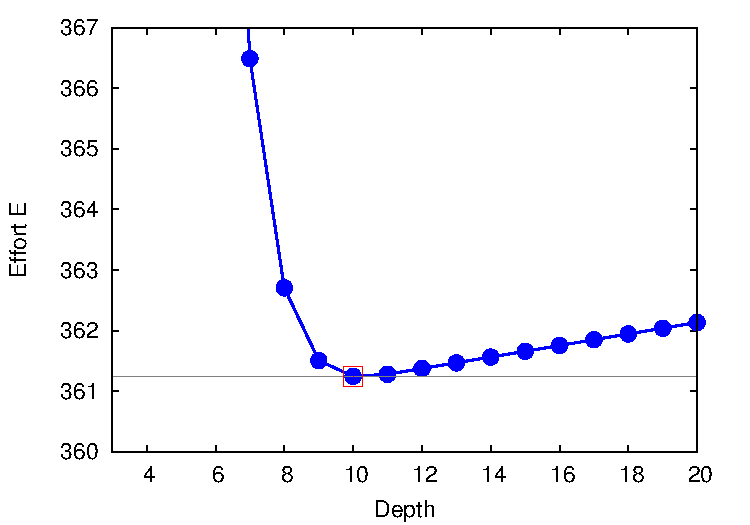
\includegraphics[width=10cm,draft=false]{immagini/effVSdepth_1000_1.pdf}
\end{figure}
\end{frame}

%--------------------------------------------------------------
\begin{frame}[noframenumbering]{The functional $\boldsymbol{\Ee}$}{Minimal Effort model (mean field model)}
\begin{figure}[ht]%
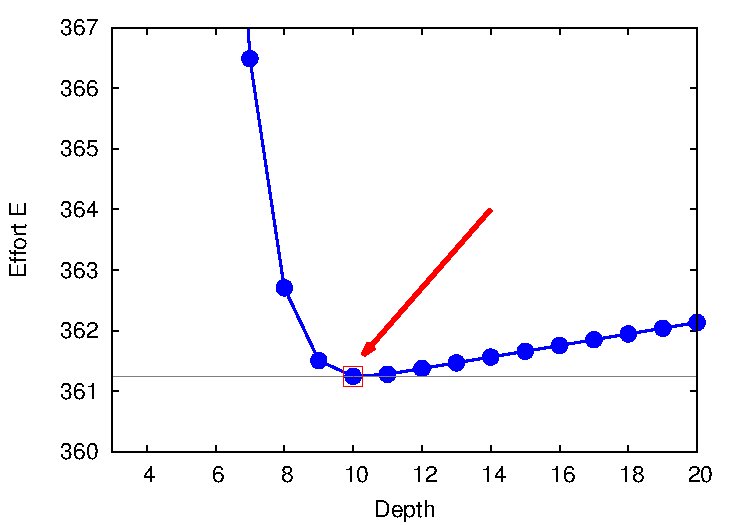
\includegraphics[width=10cm,draft=false]{immagini/Eff2.pdf}
\end{figure}
\end{frame}

%--------------------------------------------------------------
\begin{frame}{Depth VS Size is logarithmic}{Minimal Effort model (mean field model)}
\begin{figure}[p]%
\center
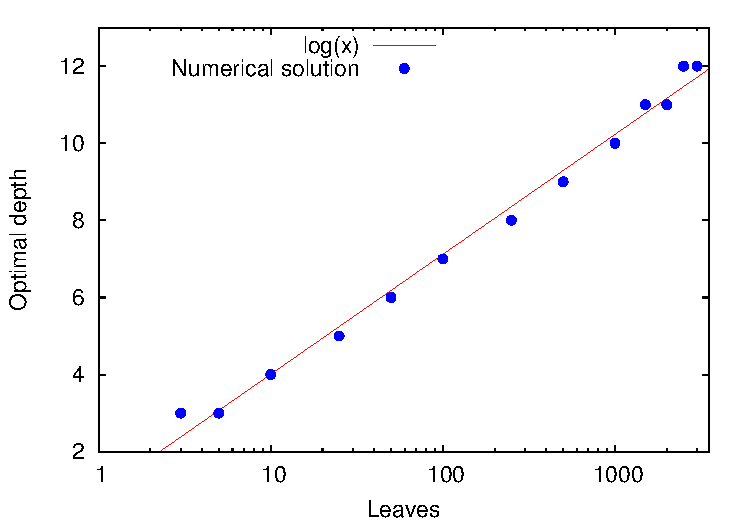
\includegraphics[width=10cm,draft=false]{immagini/depVSNnodes_eff.pdf}
\end{figure}
\end{frame}

%--------------------------------------------------------------
\begin{frame}{Shareability of the code}{Minimal Effort model (mean field model)}
\begin{figure}[p]%
\center
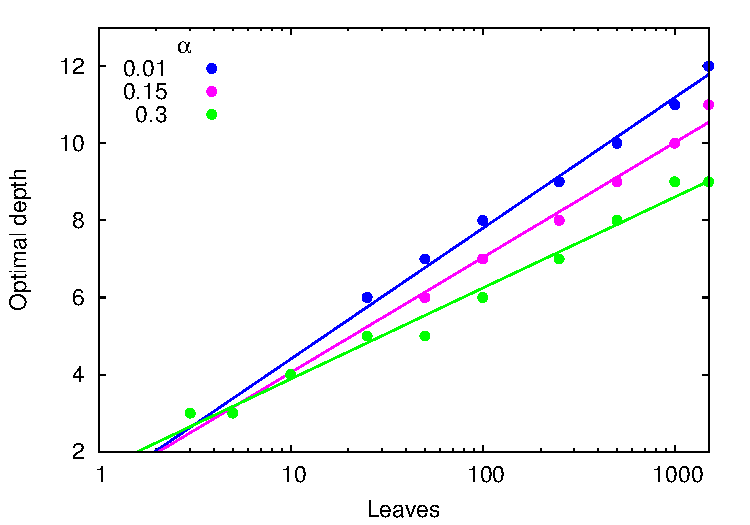
\includegraphics[width=10cm,draft=false]{immagini/Alpha.pdf}
\end{figure}
\end{frame}

%--------------------------------------------------------------
\begin{frame}[noframenumbering]{Depth VS Size is logarithmic}{Data Analysis - Comparison among languages}
\begin{figure}[H]%
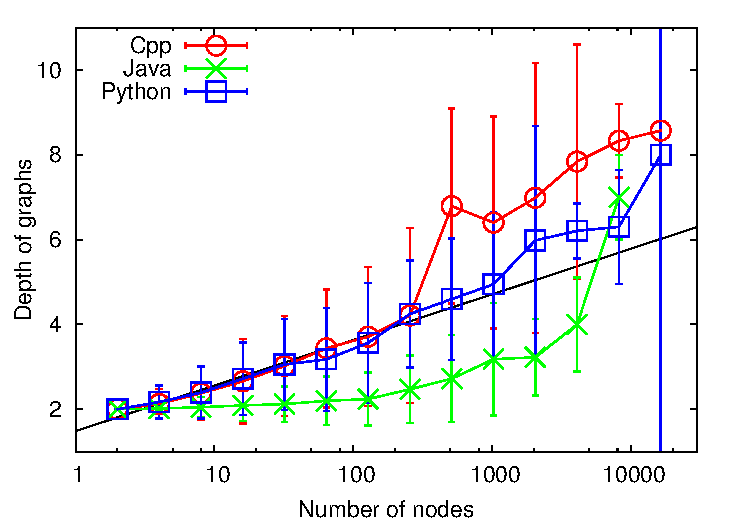
\includegraphics[width=10cm,draft=false]{immagini/depVSNnodes_err.pdf}
\end{figure}
\end{frame}

%--------------------------------------------------------------
\begingroup
\setbeamercolor{background canvas}{bg=black}
\begin{frame}[plain,noframenumbering]
\center
\textbf {\Huge {\color{white} {Hierarchies structures}}}

\end{frame}
\endgroup

%--------------------------------------------------------------
\begin{frame}{Mean outdegree grows close to the root}%{Sharing Tree model (microscopic model)}
\begin{tcolorbox}[colframe=PaleVioletRed]
\center
 Sharing Tree model
\end{tcolorbox}
\begin{figure}[p]%
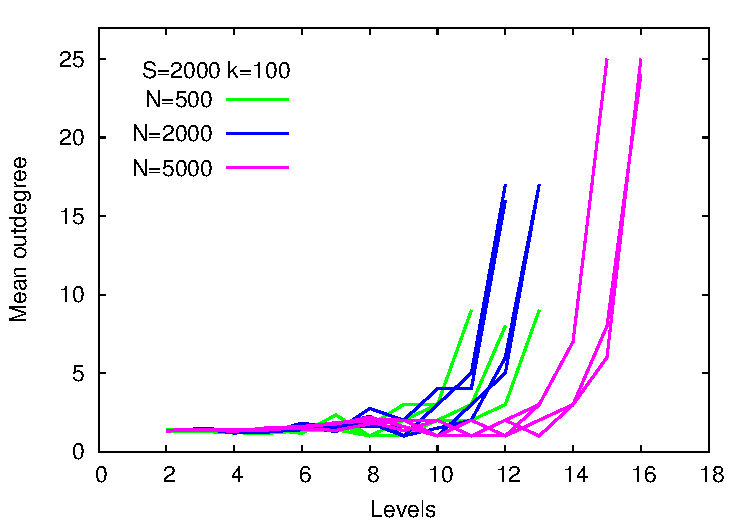
\includegraphics[width=9cm,draft=false]{immagini/ST_OvsD.pdf}
\end{figure}
\end{frame}

%--------------------------------------------------------------
\begin{frame}{Mean outdegree grows close to the root}%{Data Analysis - C++}
\begin{tcolorbox}[colframe=red]
\center
 C++
\end{tcolorbox}
\begin{figure}[ht]%
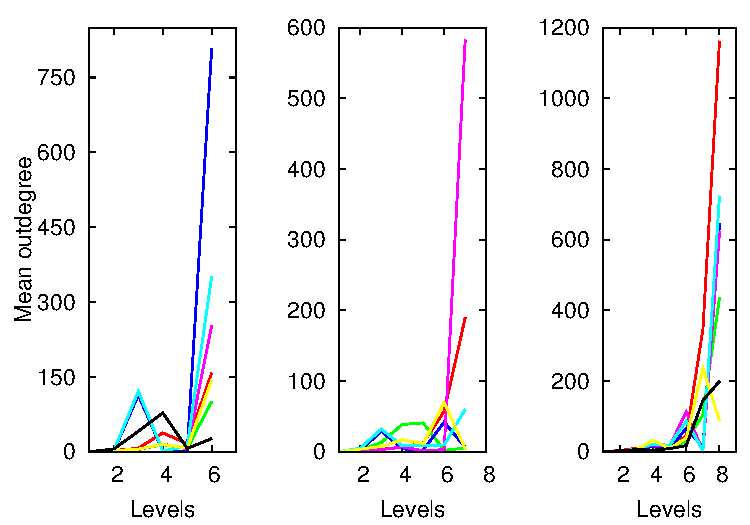
\includegraphics[width=9cm,draft=false]{immagini/CPP_OvsD.pdf}
\end{figure}\end{frame}
%--------------------------------------------------------------
\begin{frame}[noframenumbering]{Mean outdegree grows close to the root}%{Data Analysis - Java}
\begin{tcolorbox}[colframe=green]
\center
 Java
\end{tcolorbox}
\begin{figure}[hp]%
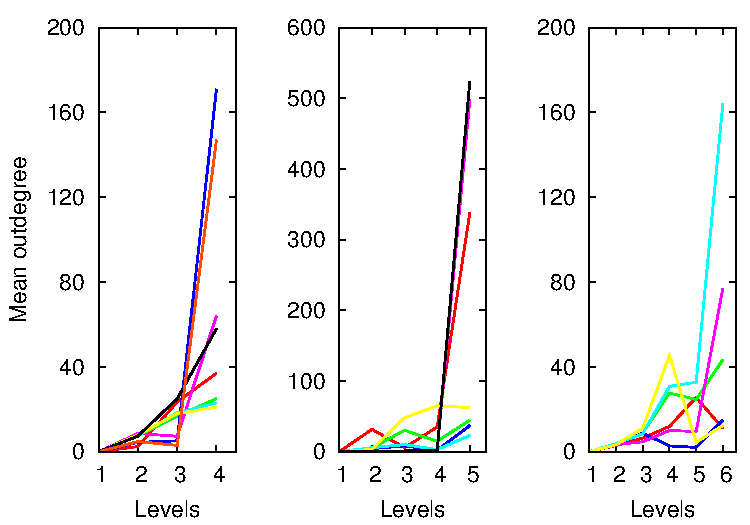
\includegraphics[width=9cm,draft=false]{immagini/JAVA_OvsD.pdf}
\end{figure}
\end{frame}
%--------------------------------------------------------------
\begin{frame}[noframenumbering]{Mean outdegree grows close to the root}%{Data Analysis - Python}
\begin{tcolorbox}[colframe=blue]
\center
 Python
\end{tcolorbox}
\begin{figure}[hp]%
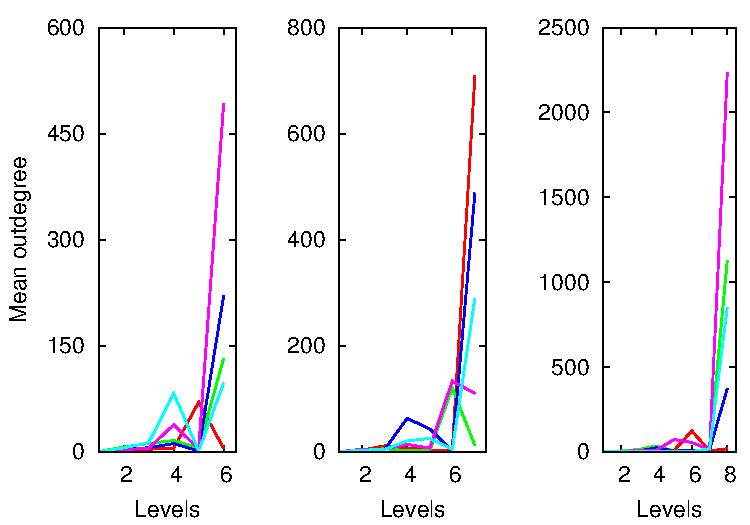
\includegraphics[width=9cm,draft=false]{immagini/PY_OvsD.pdf}
\end{figure}
\end{frame}
%--------------------------------------------------------------
\begin{frame}{Is shallow better?}%{Minimal Effort model (mean field model)}
\begin{tcolorbox}[colframe=SkyBlue]
\center
 Minimal Effort model
\end{tcolorbox}
\begin{figure}[p]%
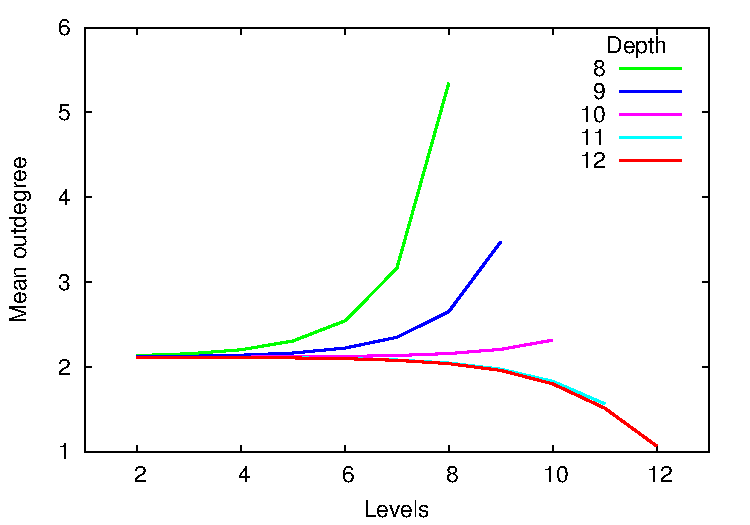
\includegraphics[width=9cm,draft=false]{immagini/EM_OvsD.pdf}
\end{figure}
\end{frame}

%--------------------------------------------------------------
\begingroup
\setbeamercolor{background canvas}{bg=black}
\begin{frame}[plain,noframenumbering]
\center
\textbf {\Huge {\color{white} {Conclusions}}}

\end{frame}
\endgroup

%--------------------------------------------------------------
\begin{frame}{Conclusions}
\begin{itemize}
\item Different OO programming languages show \textbf{\underline{common behaviors}} (in sizes distribution, outdegree distribution, depth VS size, \dots)

\item The two different \textbf{\underline{models}} (microscopic and mean field) are compatible
\item Hierarchies arise from a mechanism of \textbf{\underline{competition}} between the sake of the reuse and the difficulty of the abstraction
\item We have an interpretation about the \textbf{\underline{shallow hierarchies}} in Java
\item Both models predict the growth of the \textbf{\underline{mean outdegree}} close to the root
\item We argue that depths are \textbf{\underline{sub-optimal}}

\end{itemize}
\end{frame}

%--------------------------------------------------------------
\begingroup
\setbeamercolor{background canvas}{bg=black}
\begin{frame}[plain,noframenumbering]
\center
\textbf {\Huge {\color{white} {Extras}}}

\end{frame}
\endgroup

%--------------------------------------------------------------
\begin{frame}[noframenumbering]{Sizes distribution}{Extra}
\begin{figure}[p]%
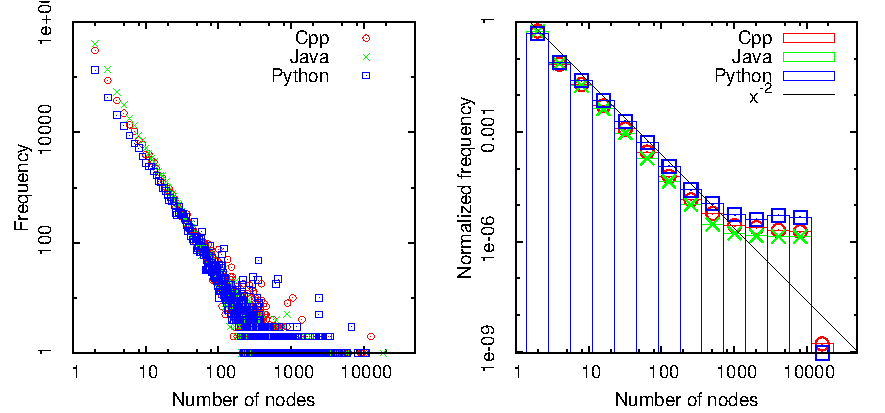
\includegraphics[width=12cm,draft=false]{immagini/fDNnodes.pdf}
\end{figure}
\end{frame}
%--------------------------------------------------------------
\begin{frame}[noframenumbering]{Outdegrees distribution}{Extra}
\begin{figure}[p]%
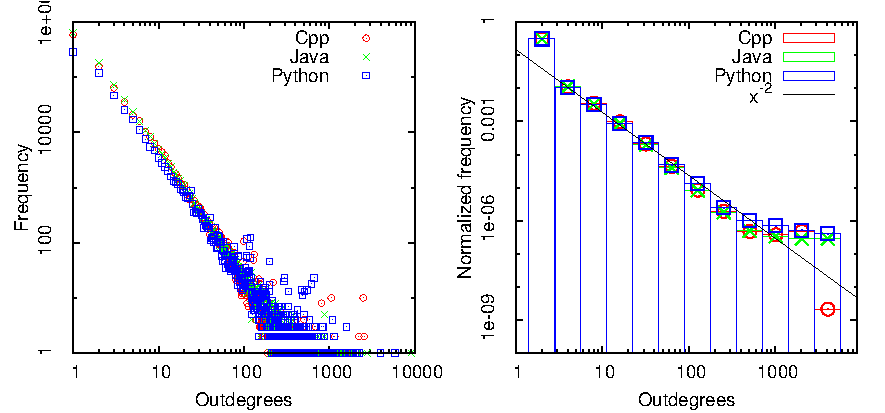
\includegraphics[width=12cm,draft=false]{immagini/fDoutdeg.pdf}
\end{figure}
\end{frame}
%--------------------------------------------------------------
\begin{frame}[noframenumbering]{Indegrees distribution}{Extra}
\begin{figure}[p]%
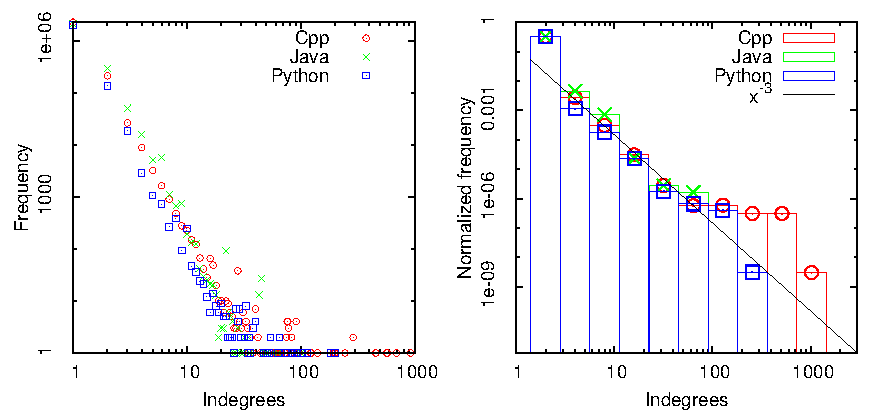
\includegraphics[width=12cm,draft=false]{immagini/fDindeg.pdf}
\end{figure}
\end{frame}
%--------------------------------------------------------------
\begin{frame}[noframenumbering]{Tree Approximation - Java}{Extra}
\begin{figure}[p]%
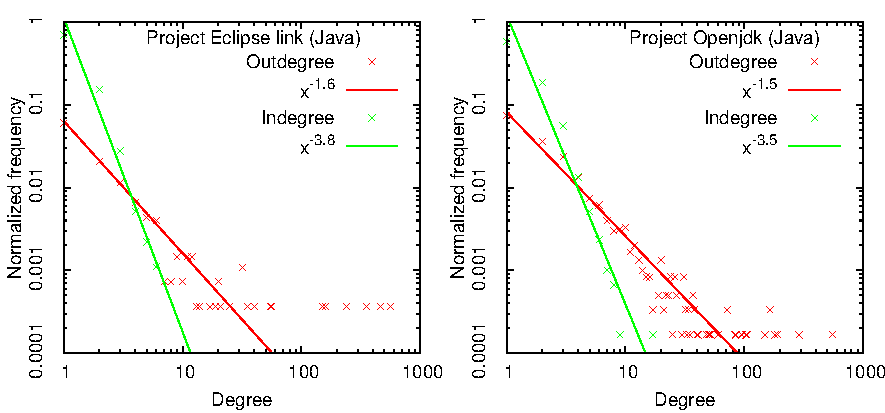
\includegraphics[width=12cm,draft=false]{immagini/javainout.pdf}
\end{figure}
\end{frame}
%--------------------------------------------------------------
\begin{frame}[noframenumbering]{Tree Approximation - Python}{Extra}
\begin{figure}[p]%
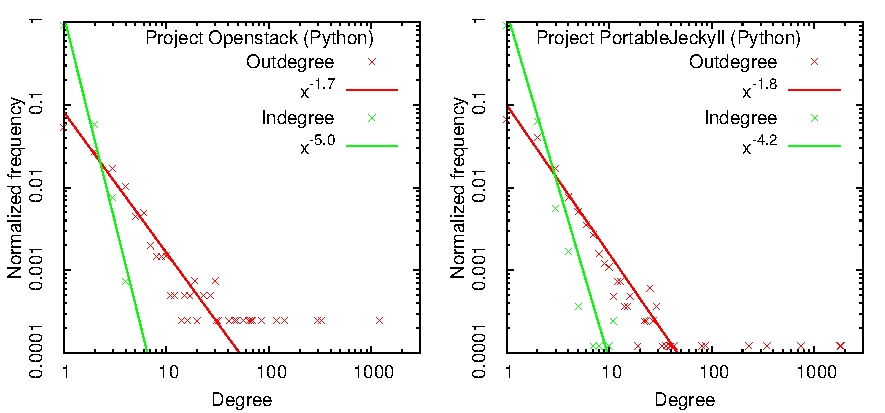
\includegraphics[width=12cm,draft=false]{immagini/pyinout.pdf}
\end{figure}
\end{frame}
%--------------------------------------------------------------
\begin{frame}[noframenumbering]{Tree Approximation - C++}{Extra}
\begin{figure}[p]%
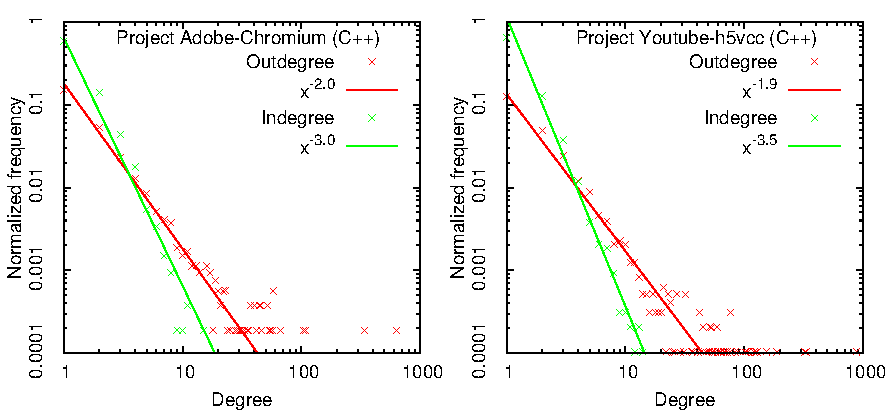
\includegraphics[width=12cm,draft=false]{immagini/cppinout.pdf}
\end{figure}
\end{frame}
%--------------------------------------------------------------
\begin{frame}[noframenumbering]{Abstractability in Sharing Tree model}{Extra}
\begin{figure}[p]%
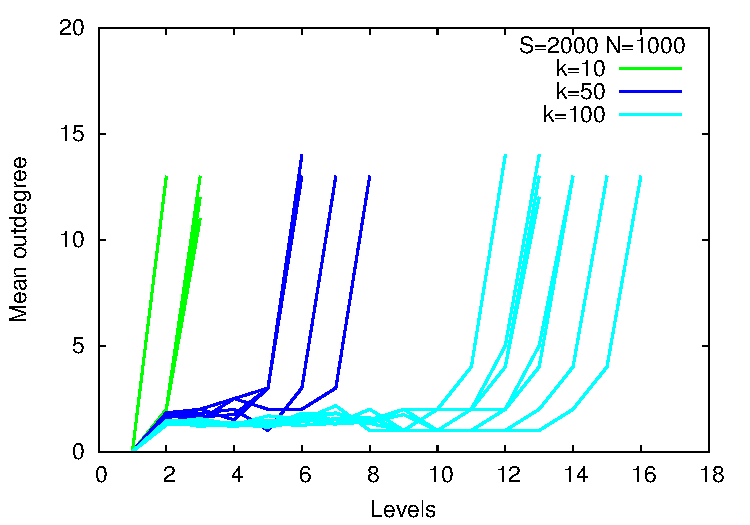
\includegraphics[width=10cm,draft=false]{immagini/extra_treekappa.pdf}
\end{figure}
\end{frame}
%--------------------------------------------------------------
\begin{frame}[noframenumbering]{Most common symbol in Sharing Tree model 1/3}{Extra}
Probability to find a selected symbol in one sequence is
\[ p = \frac{\binom{\Esse-1}{\kappa-1}}{\binom{\Esse}{\kappa}}= \frac{\kappa!(\Esse -1)!}{\Esse!(\kappa -1)!} \]
Probability that $w$ classes contain a selected symbol with
\[ Pr(w) = \binom{\Enne}{w} \, p^{w} \, (1-p)^{\Enne-w} \]

Each symbol $s \in \Esse$ appears in $w_s$ classes. The set $\{w_s\}_{s=1}^{\Esse}$ contains $\Esse$ IIDRV. The most common symbol is the one that appears $\omega$ times
\[ \omega = \max \left\{ w_1, \dots, w_{\Esse} \right\} \]
\end{frame}

\begin{frame}[noframenumbering]{Most common symbol in Sharing Tree model 2/3}{Extra}
Consider the cumulative distribution function of $\omega$
\[ F_{\omega} (y)= Pr(\omega \leq y) \]
Since $\omega$ is the maximal occurrence and $w_s$ are independent
\begin{align*}
Pr(\omega \leq y) &= Pr(w_1 \leq y, w_2 \leq y, \dots, w_{\Esse} \leq y) \\
&= Pr(w_1 \leq y) Pr(w_2 \leq y) \dots Pr(w_{\Esse} \leq y)
\end{align*}
and since all $w_s$ have the same cumulative mass function
\[ F_{\omega} (y) = F_{w}^{\Esse} (y) \]

The probability distribution of $\omega$
\begin{align*}
Pr (y = \omega) &= Pr (\omega \leq y) - Pr (\omega \leq y-1) \\
&= F_w^{\Esse} (y) - F_w^{\Esse} (y-1)
\end{align*}
\end{frame}

\begin{frame}[noframenumbering]{Most common symbol in Sharing Tree model 3/3}{Extra}
Remembering that $w_s$ are binomial random variables, the occurrence $\omega$ of the most common symbol is therefore distributed as 
\[\Psi (\omega) = \left( \sum_{i=0}^{ \omega} \text{Bin}(\Enne, i) \right)^{\Esse}- \left( \sum_{i=0}^{\omega -1} \text{Bin}(\Enne, i) \right)^{\Esse}\]

Making explicit the formula of the Binomial distribution
\[\Psi (\omega) = \left( \sum_{i=0}^{ \omega} \binom{\Enne}{i} p^i (1-p)^{\Enne -i} \right) ^{\Esse}- \left( \sum_{i=0}^{\omega -1} \binom{\Enne}{i} p^i (1-p)^{\Enne -i}\right) ^{\Esse} \]

The mean of the distribution is
\[ \langle \omega \rangle =  \Enne - \sum_{j=0}^{\Enne -1} \left( \sum_{k=0}^{j} \binom{N}{k} p^k (1-p)^{\Enne -k} \right)^\Esse \]
\end{frame}

%--------------------------------------------------------------
\begin{frame}[noframenumbering]{Most common symbol distribution}{Extra}
\begin{figure}[p]%
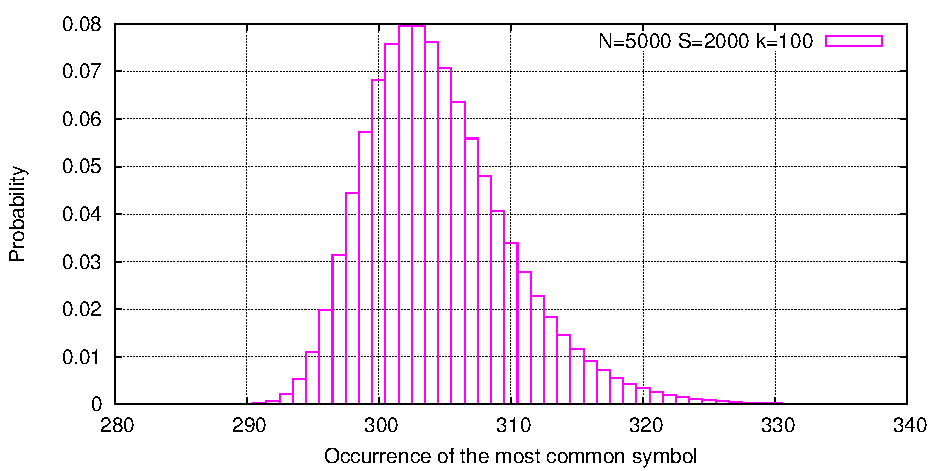
\includegraphics[width=12cm,draft=false]{immagini/campana1.pdf}
\end{figure}
\end{frame}


\begin{frame}[noframenumbering]{Sharing Tree process}{Extra}
The mean number of elements of a group at each step $t$ is given by
\[ f(x_t, t) = x_t - \sum_{j=0}^{x_t-1} \left( \sum_{i=0}^{j} \binom{x_t}{i} \Pi_t^i \left( 1 - \Pi_t \right)^{x_t-i} \right)^{\Esse-t} \]
where $\Pi_t$ is obtained with the hypergeometric distribution and considering that if a symbol has been used as \textit{the most common} then it cannot be reused, and so at each step $\Esse \to \Esse -1$ and $\kappa \to \kappa -1$.
\[ \Pi_t = \frac{\binom{\Esse-1-t}{k-1-t}}{\binom{\Esse-t}{\kappa-t}} = \frac{\Gamma(\Esse-t)\Gamma(\kappa-t+1)}{\Gamma(\kappa-t)\Gamma(\Esse-t+1)}\]

The process for the mean number of elements can so be defined as
\[ x_{t+1} = f(x_{t},t) \]
where $x_0=x(0)$ and is equal to $\Enne$ for the main process.

\end{frame}

%--------------------------------------------------------------
\begin{frame}[noframenumbering]{Null model 1}{Extra}
\begin{figure}[p]%
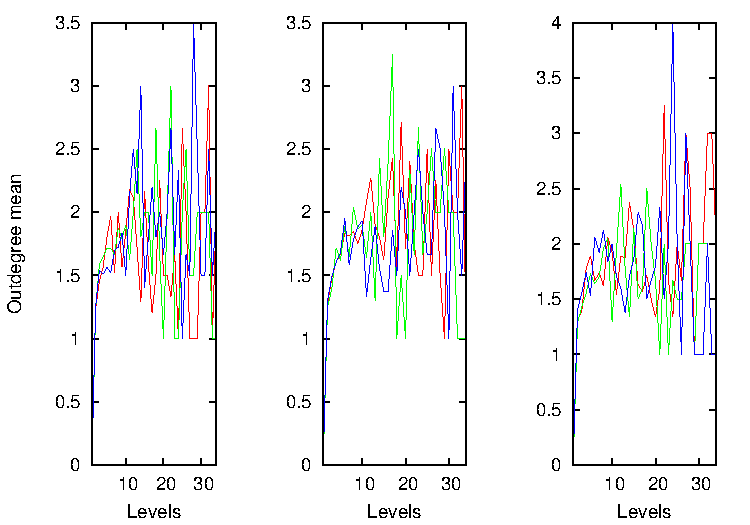
\includegraphics[width=10cm,draft=false]{immagini/Coutdeg_yul.pdf}
\end{figure}
\end{frame}

%--------------------------------------------------------------
\begin{frame}[noframenumbering]{Null model 2}{Extra}
\begin{figure}[p]%
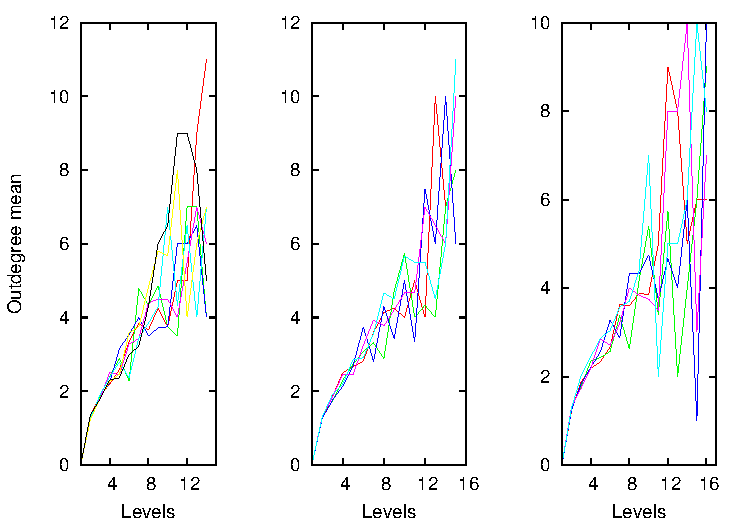
\includegraphics[width=10cm,draft=false]{immagini/Coutdeg_rus.pdf}
\end{figure}
\end{frame}
%--------------------------------------------------------------
\end{document}
